%\documentclass[crop,tikz,multi=false]{standalone}
\documentclass[crop,tikz,convert={outext=.svg,command=\unexpanded{pdf2svg \infile\space\outfile}},multi=false]{standalone}
\usepackage{amsmath}
\usepackage{amssymb}
\usepackage{mathtools}
\usepackage{fullpage}
\usepackage[T1]{fontenc}
\usepackage{lmodern}
\usepackage{tikz}
\usetikzlibrary{calc,intersections,through,backgrounds}
\usetikzlibrary{bayesnet}
\usepackage{tikzscale}
\usepackage{tkz-euclide}
\usepackage{tcolorbox}
\tcbuselibrary{skins,breakable}
% pgfplots
\usepackage{pgfplots}
\pgfplotsset{compat=1.8}
% For entities in text
\newcommand{\entity}[1]{\texttt{#1}}
% For entities in pgfplots
\newcommand{\entpgf}[1]{\texttt{#1}}

\begin{document}
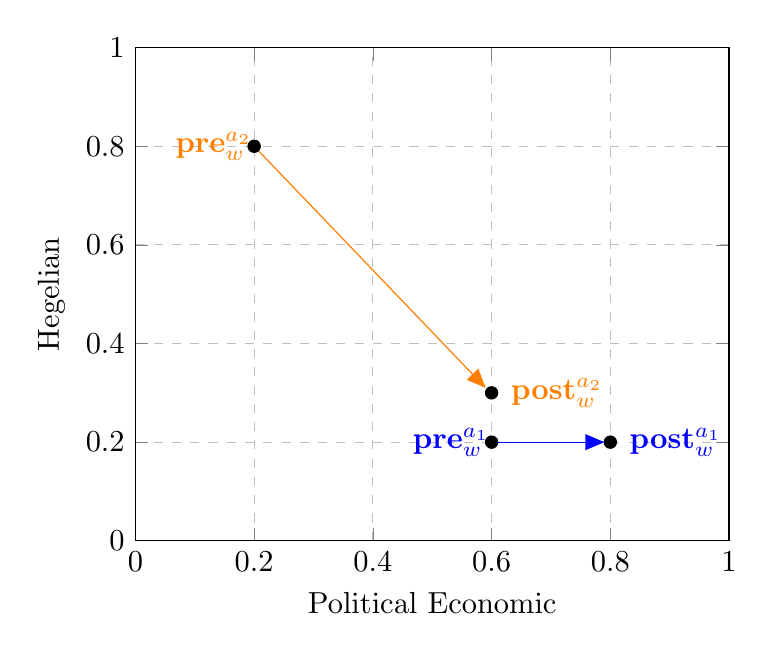
\begin{tikzpicture}[scale=1.1]
	\begin{axis}[
		%title={Temperature dependence of CuSO\(_4\cdot\)5H\(_2\)O solubility},
		xlabel={Political Economic},
		ylabel={Hegelian},
		xmin=0, xmax=1.0,
		ymin=0, ymax=1.0,
		xtick={0,0.2,0.4,0.6,0.8,1.0},
		ytick={0,0.2,0.4,0.6,0.8,1.0},
		legend pos=north west,
		ymajorgrids=true,
		xmajorgrids=true,
		grid style=dashed,
		]
		
		\addplot[
		color=blue,
		%mark=circle,
		->,
		smooth
		%patch,
		%mesh,% without mesh, pgfplots tries to fill
		%patch type=quadratic spline
		]
		coordinates {
			(0.6,0.2)(0.79,0.2)
		};
		%\legend{CuSO\(_4\cdot\)5H\(_2\)O}
		\addplot[
		color=orange,
		%mark=circle,
		->,
		smooth
		]
		coordinates {
			(0.2,0.8)(0.59,0.31)
		};
		
		\addplot[
		scatter/classes={a={blue}, b={orange}},
		%scatter/classes={%
			%	a={mark=square*,blue},%
			%	b={mark=triangle*,red},%
			%	c={mark=o,draw=black}},
		scatter, mark=*, only marks, 
		scatter src=explicit symbolic,
		nodes near coords*={\Label},
		nodes near coords style={
			%anchor=west,
			anchor=\perpointanchor,
			xshift=1mm,
			yshift=\perpointyshift,
			color=\perpointcolor
		},
		visualization depends on={value \thisrow{label} \as \Label},
		visualization depends on={value \thisrow{anchorclass} \as \perpointanchor},
		visualization depends on={value \thisrow{yshift} \as \perpointyshift},
		visualization depends on={value \thisrow{class} \as \perpointcolor}
		] table [meta=class] {
			x y anchorclass yshift class label
			0.6 0.2 east 0cm blue $\mathbf{pre}_w^{a_1}$
			0.8 0.2 west 0cm blue $\mathbf{post}_w^{a_1}$
			0.2 0.8 east 0cm orange $\mathbf{pre}_w^{a_2}$
			0.6 0.3 west 0cm orange $\mathbf{post}_w^{a_2}$
			%0.7 0.6 a C
			%0.35 0.4 a D
		};
		
	\end{axis}
\end{tikzpicture}
\end{document}
